% Options for packages loaded elsewhere
\PassOptionsToPackage{unicode}{hyperref}
\PassOptionsToPackage{hyphens}{url}
\PassOptionsToPackage{dvipsnames,svgnames,x11names}{xcolor}
%
\documentclass[
  ignorenonframetext,
]{beamer}
\usepackage{pgfpages}
\setbeamertemplate{caption}[numbered]
\setbeamertemplate{caption label separator}{: }
\setbeamercolor{caption name}{fg=normal text.fg}
\beamertemplatenavigationsymbolsempty
% Prevent slide breaks in the middle of a paragraph
\widowpenalties 1 10000
\raggedbottom
\setbeamertemplate{part page}{
  \centering
  \begin{beamercolorbox}[sep=16pt,center]{part title}
    \usebeamerfont{part title}\insertpart\par
  \end{beamercolorbox}
}
\setbeamertemplate{section page}{
  \centering
  \begin{beamercolorbox}[sep=12pt,center]{part title}
    \usebeamerfont{section title}\insertsection\par
  \end{beamercolorbox}
}
\setbeamertemplate{subsection page}{
  \centering
  \begin{beamercolorbox}[sep=8pt,center]{part title}
    \usebeamerfont{subsection title}\insertsubsection\par
  \end{beamercolorbox}
}
\AtBeginPart{
  \frame{\partpage}
}
\AtBeginSection{
  \ifbibliography
  \else
    \frame{\sectionpage}
  \fi
}
\AtBeginSubsection{
  \frame{\subsectionpage}
}
\usepackage{amsmath,amssymb}
\usepackage{iftex}
\ifPDFTeX
  \usepackage[T1]{fontenc}
  \usepackage[utf8]{inputenc}
  \usepackage{textcomp} % provide euro and other symbols
\else % if luatex or xetex
  \usepackage{unicode-math} % this also loads fontspec
  \defaultfontfeatures{Scale=MatchLowercase}
  \defaultfontfeatures[\rmfamily]{Ligatures=TeX,Scale=1}
\fi
\usepackage{lmodern}
\ifPDFTeX\else
  % xetex/luatex font selection
\fi
% Use upquote if available, for straight quotes in verbatim environments
\IfFileExists{upquote.sty}{\usepackage{upquote}}{}
\IfFileExists{microtype.sty}{% use microtype if available
  \usepackage[]{microtype}
  \UseMicrotypeSet[protrusion]{basicmath} % disable protrusion for tt fonts
}{}
\makeatletter
\@ifundefined{KOMAClassName}{% if non-KOMA class
  \IfFileExists{parskip.sty}{%
    \usepackage{parskip}
  }{% else
    \setlength{\parindent}{0pt}
    \setlength{\parskip}{6pt plus 2pt minus 1pt}}
}{% if KOMA class
  \KOMAoptions{parskip=half}}
\makeatother
\usepackage{xcolor}
\newif\ifbibliography
\usepackage{longtable,booktabs,array}
\usepackage{calc} % for calculating minipage widths
\usepackage{caption}
% Make caption package work with longtable
\makeatletter
\def\fnum@table{\tablename~\thetable}
\makeatother
\setlength{\emergencystretch}{3em} % prevent overfull lines
\providecommand{\tightlist}{%
  \setlength{\itemsep}{0pt}\setlength{\parskip}{0pt}}
\setcounter{secnumdepth}{5}
\usepackage{/home/jb/R/x86_64-pc-linux-gnu-library/4.4/quack/rmarkdown/templates/presentation/resources/beamerthemeAustin}
\usepackage{/home/jb/R/x86_64-pc-linux-gnu-library/4.4/quack/rmarkdown/templates/presentation/resources/beamercolorthemelonghorn}
\newcommand{\setsep}{\setlength{\itemsep}{3pt}}
\newcommand{\setskip}{\setlength{\parskip}{3pt}}
\renewcommand{\tightlist}{\setsep\setskip}
\newcommand{\expectation}[1]{\ensuremath{\mathbb{E}\left[#1\right]}}
\newcommand{\pd}[2][]{\ensuremath{\frac{\partial{#1}}{\partial{#2}}}}
\DeclareMathOperator{\Var}{Var}
\DeclareMathOperator{\Cov}{Cov}
\newcommand{\variance}[1]{\ensuremath{\Var\left[#1\right]}}
\newcommand{\covariance}[1]{\ensuremath{\Cov\left[#1\right]}}
\DeclareMathOperator{\standarddeviation}{sd}
\DeclareMathOperator{\standarderror}{se}
\usepackage{siunitx}
\ifLuaTeX
  \usepackage{selnolig}  % disable illegal ligatures
\fi
\usepackage{bookmark}
\IfFileExists{xurl.sty}{\usepackage{xurl}}{} % add URL line breaks if available
\urlstyle{same}
\hypersetup{
  pdftitle={Statistical Analysis in Political Science II:Violations of independence},
  pdfauthor={JBrandon Duck-Mayr},
  colorlinks=true,
  linkcolor={Maroon},
  filecolor={Maroon},
  citecolor={Blue},
  urlcolor={Blue},
  pdfcreator={LaTeX via pandoc}}

\title{Statistical Analysis in Political Science II:\newline Violations of independence}
\author{JBrandon Duck-Mayr}
\date{March 12, 2025}

\begin{document}
\frame{\titlepage}

\begin{frame}{Assumptions, assumptions}
\phantomsection\label{assumptions-assumptions}
Recall the assumptions of the classical linear model:

\pause

\begin{enumerate}
\tightlist
\item
  Linear in parameters
\item
  Random sampling
\item
  No perfect collinearity
\item
  Zero conditional mean: The error term has the same expected value at any value of the explanatory variables: \(\ensuremath{\mathbb{E}\left[\varepsilon \mid x_1, \dots, x_k\right]} = 0\)
\item
  Homoscedasticity: The error term has the same variance at any value of the explanatory variables; \(\ensuremath{\mathop{\mathrm{Var}}\left[\varepsilon \mid x_1, \dots, x_k\right]} = \sigma^2\)
\item
  \(\varepsilon \sim \mathcal{N}\left( 0, \sigma^2 \right)\)
\end{enumerate}

\pause

What happens when we don't have random sampling?
\end{frame}

\begin{frame}{Time series data}
\phantomsection\label{time-series-data}
\pause

\begin{itemize}[<+->]
\tightlist
\item
  Each observation \emph{temporally follows} the previous observation
\item
  So \emph{necessarily}, random sampling is violated
\end{itemize}
\end{frame}

\begin{frame}{Finite distributed lag models}
\phantomsection\label{finite-distributed-lag-models}
\pause

\begin{itemize}[<+->]
\tightlist
\item
  Our predictors may have a lagged effect
\item
  So just include lagged values of the predictor;
  this is called a finite distributed lag (FDL) model
\item
  For a \emph{one} period increase in the predictor

  \begin{itemize}[<+->]
  \tightlist
  \item
    Coefficient on contemporaneous value is the contemporaneous effect, or the \emph{impact propensity}
  \item
    The coefficient on the first lag is the effect on the outcome in the next period after a one-period increase, etc
  \end{itemize}
\item
  For a \emph{permanent} increase

  \begin{itemize}[<+->]
  \tightlist
  \item
    Coefficient on contemporaneous value is still the contemporaneous effect
  \item
    But now the effect in the next period is the contemporaneous coefficient \emph{plus} the coefficient on the first lag, etc

    \begin{itemize}[<+->]
    \tightlist
    \item
      Sum of coefficients for \(h\) periods is the \emph{cumulative effect}
    \item
      Sum of all lag coefficients is called the \emph{long-run propensity} or \emph{long-run multiplier}
    \end{itemize}
  \end{itemize}
\end{itemize}
\end{frame}

\begin{frame}{More assumptions}
\phantomsection\label{more-assumptions}
\begin{itemize}
    \setlength{\itemsep}{3pt}\setlength{\parskip}{3pt}
    \item[TS1]<2-> Linearity in parameters (essentially the same as MLR1)
    \item[TS2]<3-> No perfect collinearity (essentially the same as MLR2)
    \item[TS3]<4-> Zero conditional mean: $\mathbb{E}\left(\varepsilon_t\mid\mathbf{X}\right) = 0, t = 1, 2, \dots n$
    \begin{itemize}
        \setlength{\itemsep}{3pt}\setlength{\parskip}{3pt}
        \item<5-> Analog of MLR4, obviates the need for random sampling
        \item<6-> Error term at time $t$ is uncorrelated with predictors in \textbf{every} time period
        \item<7-> \textit{contemporaneous exogeneity} only requires $\mathbb{E}\left(\varepsilon_t\mid\mathbf{x}_t\right) = 0$
        \item<8-> Assumption TS3 goes farther and is called \textit{strict exogeneity}
        \item<9-> Note this does not require lack of correlation of errors
        \item<10-> This can fail under omitted variable bias or when there's feedback between the error and a predictor
    \end{itemize}
    \item[TS4]<11-> Homoscedasticity: $\text{Var}\left(\varepsilon_t\mid\mathbf{X}\right) = \text{Var}\left(\varepsilon_t\right) = \sigma^2, t = 1, 2, \dots, n$
    \item[TS5]<12-> No serial correlation: Conditional on $\mathbf{X}$, the errors in two time periods are uncorrelated: $\text{Cor}\left(\varepsilon_t,\varepsilon_s\mid\mathbf{X}\right) = 0,\,\forall\,\, t \neq s$
\end{itemize}
\end{frame}

\begin{frame}{What do they buy us?}
\phantomsection\label{what-do-they-buy-us}
\pause

\begin{itemize}[<+->]
\tightlist
\item
  Under assumptions TS1--TS3, OLS is unbiased
\item
  If we have contemporaneous exogeneity instead of TS3, OLS is still consistent, but not unbiased
\item
  Under assumptions TS1--TS5, we get the sampling variance of \(\hat{\beta}\): \(\text{Var}\left(\hat{\boldsymbol\beta}\mid\mathbf{X}\right) = \sigma^2\left(\mathbf{X'X}\right)^{-1}\) (same as in cross-sectional)
\item
  Under assumptions TS1--TS5, \(\hat{\sigma}^2 = \text{SSR}/df\) is an unbiased estimator of \(\sigma^2\)
\item
  Under assumptions TS1--TS5, OLS is BLUE
\end{itemize}

\begin{itemize}
    \setlength{\itemsep}{3pt}\setlength{\parskip}{3pt}
    \item[TS6]<7-> Normally distributed errors
\end{itemize}

\begin{itemize}
    \setlength{\itemsep}{3pt}\setlength{\parskip}{3pt}
    \item<8-> Under assumptions TS1--TS6, OLS estimators are normally distributed, and $t$ and $F$ statistics and usual confidence intervals are all valid
\end{itemize}
\end{frame}

\begin{frame}{Time trends}
\phantomsection\label{time-trends}
\pause

\begin{itemize}[<+->]
\tightlist
\item
  Trending variables don't necessarily violate TS1--TS6
\item
  But you could end up with a spurious correlation when the trend affects both the outcome and one or more predictors
\item
  But simply adding a time trend fixes this
\item
  We can also account for seasonality using dummies
\end{itemize}
\end{frame}

\begin{frame}{Stationarity and weak dependence}
\phantomsection\label{stationarity-and-weak-dependence}
\pause

\begin{itemize}[<+->]
\tightlist
\item
  A process \(\{x_t; t = 1, 2, \dots\}\) is \textbf{stationary} if the joint distribution of \(\left(x_t, x_{t+1}, \dots x_{t + m}\right)\) is the same as the joint distribution of \(\left(x_{t+h}, x_{t+h+1}, \dots x_{t+h + m}\right)\) for all \(t\), \(m\), and \(h\)
\item
  A stationary time series is a \textbf{weakly dependent} process ``if \(x_t\) and \(x_{t+h}\) are `almost independent' as \(h\) increases without bound'' (Wooldridge, 368)
\item
  Weak dependence replaces random sampling for proving the LLN and CLT hold
\end{itemize}
\end{frame}

\begin{frame}{\textbf{MORE} assumptions???}
\phantomsection\label{more-assumptions-1}
\begin{itemize}
    \setlength{\itemsep}{3pt}\setlength{\parskip}{3pt}
    \item[TS1']<2-> Linearity, stationarity, and weak dependence
    \item[TS2']<3-> No perfect collinearity
    \item[TS3']<4-> Zero conditional mean: Explanatory variables are \textit{contemporaneously exogenous}; $\mathbb{E}\left(\varepsilon_t\mid\mathbf{x}_t\right) = 0$
    \item[TS4']<5-> \textit{Contemporaneous} homoscedasticity: $\text{Var}\left(\varepsilon_t\mid\mathbf{x}_t\right) = \sigma^2$
    \item[TS5']<6-> No serial correlation
\end{itemize}
\end{frame}

\begin{frame}{What do \textbf{THOSE} buy us?? (asymptotics)}
\phantomsection\label{what-do-those-buy-us-asymptotics}
\pause

\begin{itemize}[<+->]
\tightlist
\item
  Under TS1'--TS3', OLS is consistent
\item
  Under TS1'--TS5', OLS estimator is asymptotically normally distributed and \(t\) and \(F\) statistics are asymptotically valid
\end{itemize}
\end{frame}

\begin{frame}{Autoregressive processes}
\phantomsection\label{autoregressive-processes}
\pause

\begin{itemize}[<+->]
\tightlist
\item
  Now think about if \[ y_t = \rho_1 y_{t-1} + e_t, t = 1, 2, \dots, n \]
\item
  If \(|\rho| < 1\), this \textbf{AR(1)} process is weakly dependent
\item
  \textbf{But} if not, it is not
\end{itemize}
\end{frame}

\begin{frame}{Persistence}
\phantomsection\label{persistence}
\begin{itemize}[<+->]
\tightlist
\item
  Difference between trend and persistence/dependence
\item
  ``Unit root''

  \begin{itemize}[<+->]
  \tightlist
  \item
    First differencing

    \begin{itemize}[<+->]
    \tightlist
    \item
      ``difference stationary process''
    \item
      Also removes any trends
    \end{itemize}
  \item
    Estimate of correlation of the outcome with its lag as an estimate of unit-root-ness

    \begin{itemize}[<+->]
    \tightlist
    \item
      BUT, de-trend first or you will overestimate the correlation
    \end{itemize}
  \end{itemize}
\end{itemize}
\end{frame}

\begin{frame}{Dynamically complete models}
\phantomsection\label{dynamically-complete-models}
\begin{itemize}[<+->]
\tightlist
\item
  A \textbf{dynamically complete model} means all lags of \(y\) and \(x\) that are needed are included
\item
  If your model is dynamically complete, TS5' is automatically satisfied
\item
  Sequential exogeneity: \(\mathbb{E}\left(\varepsilon_t\mid\mathbf{x}_t, \mathbf{x}_{t-1}, \dots\right) = \mathbb{E}\left(\varepsilon_t\right) = 0, t = 1, 2, \dots\)

  \begin{itemize}[<+->]
  \tightlist
  \item
    Strict exogeneity \(\Rightarrow\) sequential exogeneity
  \item
    Sequential exogeneity \(\Rightarrow\) contemporaneous exogeneity
  \item
    Also dynamic completeness \(\Rightarrow\) sequential exogeneity
  \item
    But, we can get sequential exogeneity without dynamic completeness, and sometimes we'll feel like that's good enough
  \end{itemize}
\end{itemize}
\end{frame}

\begin{frame}{Serially correlated errors}
\phantomsection\label{serially-correlated-errors}
\begin{itemize}[<+->]
\tightlist
\item
  Does not affect unbiasedness (which relied on strict exogeneity) or consistency (which needed TS1'--TS3')
\item
  OLS is no longer BLUE though
\item
  Moreover, test statistics and standard errors are no longer valid, even asymptotically
\end{itemize}
\end{frame}

\begin{frame}{Testing for serial correlation}
\phantomsection\label{testing-for-serial-correlation}
\begin{itemize}[<+->]
\tightlist
\item
  Under strict exogeneity

  \begin{itemize}[<+->]
  \tightlist
  \item
    Note this means no lagged DV!
  \item
    Regress residuals on lagged residuals; t-stat on rho is the test
  \item
    Durbin-Watson

    \begin{itemize}[<+->]
    \tightlist
    \item
      But requires all CLM assumptions for inference
    \item
      Can also be inconclusive
    \end{itemize}
  \end{itemize}
\item
  Without strict exogeneity

  \begin{itemize}[<+->]
  \tightlist
  \item
    Same thing, but include more residual lags
  \item
    Then do an \(F\) test for joint significance of residual lag coefficients
  \end{itemize}
\item
  What do we do about it???

  \begin{itemize}[<+->]
  \tightlist
  \item
    Newey-West (1987) standard errors
  \item
    Also called ``HAC'' standard errors
  \end{itemize}
\end{itemize}
\end{frame}

\begin{frame}{Other violations of independence}
\phantomsection\label{other-violations-of-independence}
\pause

\begin{itemize}[<+->]
\tightlist
\item
  Very closely related is \emph{spatial} autocorrelation

  \begin{itemize}[<+->]
  \tightlist
  \item
    This is more complicated than temporal autocorrelation
  \item
    Time is one dimensional and only runs in one direction, not so for space
  \item
    Tests: Moran's \emph{I}, Geary's \emph{C}
  \end{itemize}
\item
  Clusters
\end{itemize}
\end{frame}

\begin{frame}{Clustered data}
\phantomsection\label{clustered-data}
\pause

\begin{figure}
\centering
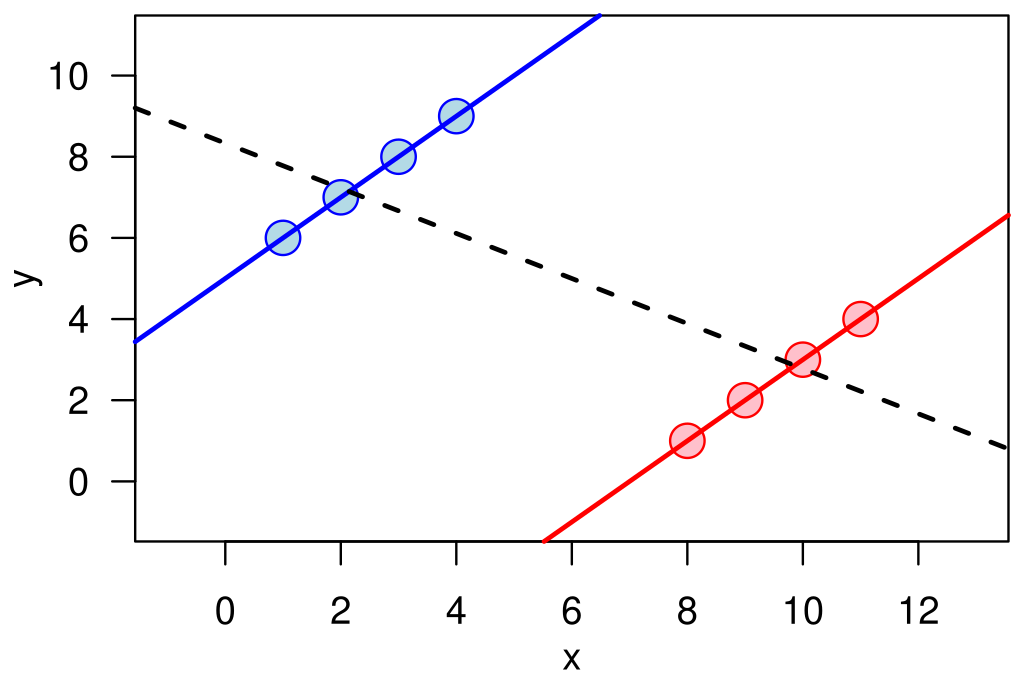
\includegraphics[width = 0.8\textwidth]{simpsons-paradox}
\end{figure}

\pause

\begin{itemize}[<+->]
\tightlist
\item
  controlling for \emph{confounders}
\item
  multi-level models
\end{itemize}
\end{frame}

\end{document}
